\documentclass[12pt]{article}
\usepackage[spanish]{babel}
\usepackage{natbib}
\usepackage{url}
\usepackage[utf8x]{inputenc}
\usepackage{amsmath}
\usepackage{float}
\usepackage{subfig}
\usepackage{graphicx}
\graphicspath{{images/}}
\usepackage{parskip}
\usepackage{fancyhdr}
\usepackage{vmargin}
\usepackage{mathtools}
\usepackage{amssymb} 



\title{Actividad \#3: Efemérides }							
\author{\Large Jesùs Valenzuela Nieblas\\}											
\date{\today} 

\makeatletter
\let\thetitle\@title
\let\theauthor\@author
\let\thedate\@date										
\makeatother

\pagestyle{fancy}

\lhead{\thetitle}
\rhead{}
\cfoot{\thepage}

\begin{document}

%%%%%%%%%%%%%%%%%%%%%%%%%%%%%%%%%%%%%%%%%%%%%%%%%%%%%%%%%%%%%%%%%%%%%%%%%%%%%%%%%%%%%%%%%

\begin{titlepage}
	\centering
    \vspace*{.5cm}
     
\includegraphics[scale = 0.7]{logo}\\	% University Logo
    \textsc{\Large Universidad de Sonora}\\[1.0 cm]	% University Name
	\textsc{\Large División de Ciencias Exactas y Naturales}\\[.50 cm]
  	\textsc{\Large Licenciatura en Fìsica}\\[.5 cm]
  \textsc{\large Fìsica Computacional 1}\\[1.5 cm]				% Course Name
	
	{ \huge \bfseries \thetitle}\\

    \vspace*{3 cm}
	\begin{minipage}{\textwidth}
    \centering
    \theauthor
	\end{minipage}\\[3 cm]
	{\large \thedate}\\[2 cm]
 
	\vfill
	
\end{titlepage}

%%%%%%%%%%%%%%%%%%%%%%%%%%%%%%%%%%%%%%%%%%%%%%%%%%%%%%%%%%%%%%%%%%%%%%%%%%%%%%%%%%%%%%%%%

\section{Introducciòn}
En la Astronomía y navegación celeste, una efemérides proporciona las posiciones de los objetos astronómicos y satélites artificiales a un determinado tiempo. Históricamente, las posiciones se han proporcionado como tablas de valores, dados en intervalos regulares de fechas y tiempos. Las efemérides modernas se obtienen de modelos matemaáticos de los movimientos de los objetos astronómicos y la Tierra. 
Las efemérides han sido publicadas a lo largo de la historia de la humanidad, siendo las primeras efemérides en la cultura griega sobre el Cometa Halley alrededor de 466 AC, en  documentos de China y Babilonia. El cometa Halley se acerca al Sol cada 76-77 años. La última aparición fue en 1986 y la próxima oportunidad de observarlo será a mediados de 2061.
\begin{figure}[H]
\centering
\includegraphics[scale=.8]{orbit}
\end{figure}
\subsection{Actividad a realizar:}
Para la creación  de los modelos matemáticos, es necesario encontrar una función que pase por todos los puntos observados. Eso se llama Interpolación.
 
Ên esta actividad actividad se pretende crear un programa que realice una interpolaciòn lineal, cuadràtica y cùbica en base al siguiente còdigo proporcionado por el maestro:
\begin{verbatim}
 
import numpy as np
import matplotlib.pyplot as plt
from scipy.interpolate import interp1d

# Original "data set" --- 21 random numbers between 0 and 1.
x0 = np.linspace(-1,1,21)
y0 = np.random.random(21)

plt.plot(x0, y0, 'o', label='Data')

# Array with points in between those of the data set for interpolation.
x = np.linspace(-1,1,101)

# Available options for interp1d
options = ('linear', 'nearest', 'zero', 'slinear', 'quadratic', 'cubic', 10)

for o in options:
    f = interp1d(x0, y0, kind=o)    # interpolation function
    plt.plot(x, f(x), label=o)      # plot of interpolated data

plt.legend()
plt.show()

\end{verbatim}
\section{Dados 10 puntos aleatorios entre $x=0$ y $x=3$ para la función $f(x) = sin(2 x).$}
\subsection{Còdigo}
\begin{verbatim}
import numpy as np
import matplotlib.pyplot as plt
from scipy.interpolate import interp1d
​
xa=np.random.random(10)
x0 = xa*3
y0 = np.sin(2*x0)
​
plt.plot(x0, y0, 'o', label='Data')
​
x = np.linspace(min(x0),max(x0),101)
​
# Available options for interp1d
options = ('linear', 'quadratic', 'cubic')
​
for o in options:
    f = interp1d(x0, y0, kind=o)   
    plt.plot(x, f(x), label=o)      
plt.legend()
plt.show()
\end{verbatim}

\subsection{Gràfica resultante}
\begin{figure}[H]
\centering
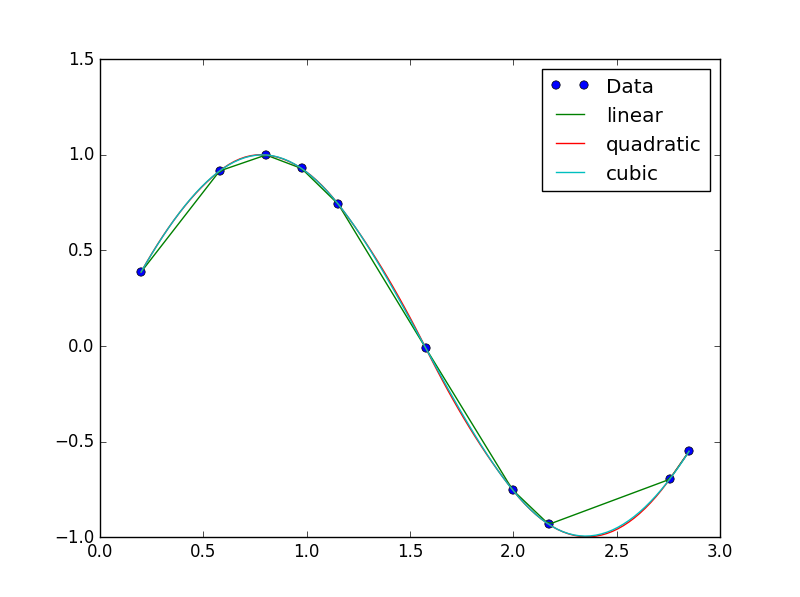
\includegraphics[scale=.8]{f1}
\end{figure}
\section{Dados 20 puntos aleatorios entre $x=-10$ y $x=10$ para la función $f(x) = sin(x)/x$}


\subsection{Còdigo}
\begin{verbatim}
import numpy as np
import matplotlib.pyplot as plt
from scipy.interpolate import interp1d

xa = np.random.random(20)
x0= (xa-(1/2))*20
y0 = np.sin(x0)/x0

plt.plot(x0, y0, 'o', label='Data')

x=np.linspace(min(x0), max(x0), 101)

options = ('linear', 'quadratic', 'cubic')

for o in options:
    f = interp1d(x0, y0, kind=o)    
    plt.plot(x, f(x), label=o)     
plt.legend()
plt.show()
\end{verbatim}

\subsection{Gràfica resultante}
\begin{figure}[H]
\centering
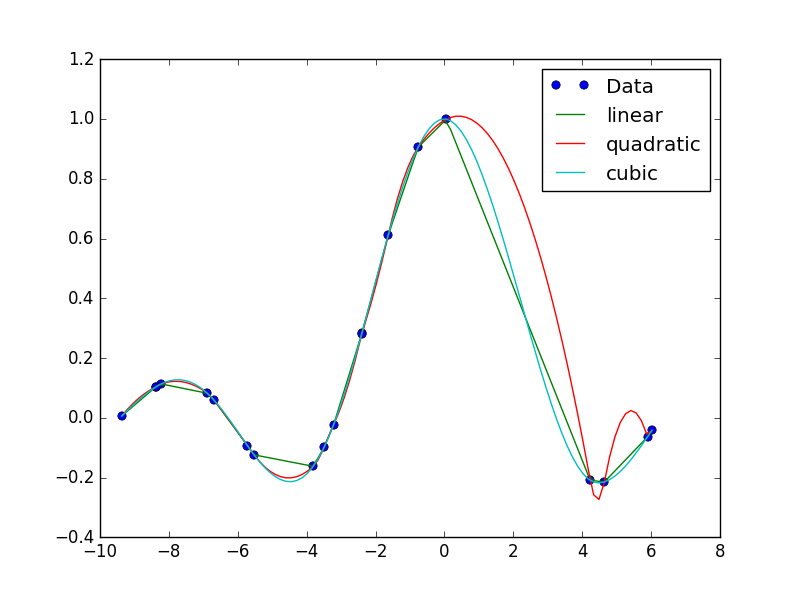
\includegraphics[scale=.8]{f2}
\end{figure}

\section{Dados 16 puntos aleatorios entre $x=-3$ y $x=3$ para la función $f(x) = x^2 sin(2 x)$}

\subsection{Còdigo}
\begin{verbatim}
import numpy as np
import matplotlib.pyplot as plt
from scipy.interpolate import interp1d

xa = np.random.random(16)
x0= (xa-(1/2))*6
y0 = (x0**2)*np.sin(2*x0)

plt.plot(x0, y0, 'o', label='Data')

x=np.linspace(min(x0), max(x0), 101)

options = ('linear', 'quadratic', 'cubic')

for o in options:
    f = interp1d(x0, y0, kind=o)    
    plt.plot(x, f(x), label=o)     
plt.legend()
plt.show()
\end{verbatim}
\subsection{Gràfica resultante}
\begin{figure}[H]
\centering
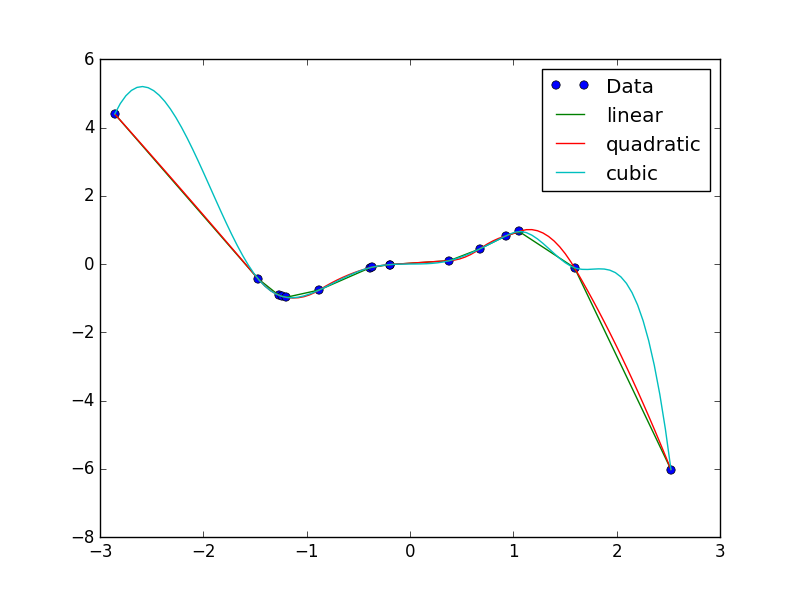
\includegraphics[scale=.8]{f3}
\end{figure}


\section{Dados 12 puntos aleatorios entre $x=-2$ y $x=2$ para la función $f(x) = x^3 sin(3 x)$}

\subsection{Còdigo}
\begin{verbatim}
import numpy as np
import matplotlib.pyplot as plt
from scipy.interpolate import interp1d

xa = np.random.random(12)
x0= (xa-(1/2))*4
y0 = (x0**3)*np.sin(x0*3)

plt.plot(x0, y0, 'o', label='Data')

x=np.linspace(min(x0), max(x0), 101)

options = ('linear', 'quadratic', 'cubic')

for o in options:
    f = interp1d(x0, y0, kind=o)    
    plt.plot(x, f(x), label=o)     
plt.legend()
plt.show()
\end{verbatim}

\subsection{Gràfica resultante}
\begin{figure}[H]
\centering
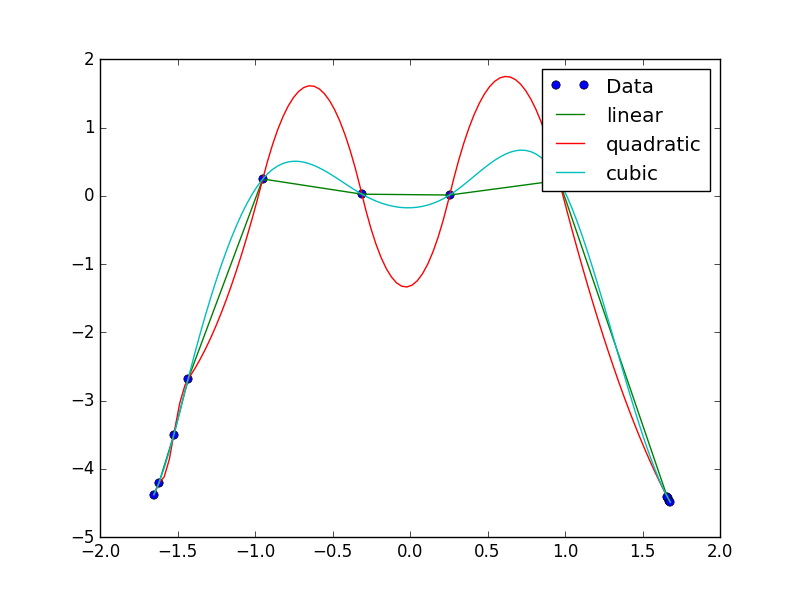
\includegraphics[scale=.8]{f4}
\end{figure}







\end{document}
